\section{Subspace Clustering}
The idea of subspace clustering is to identify the subspaces that allows better clustering. Two different approaches of subspace clustering will be discussed in this section including three algorithms: CLIQUE, MAFIA and SUBCLU.

\subsection{Grid-Based approach}
In a grid-based approach, $\mathcal{S}$ is partitioned into an axis-parallel grid structure. Each grid cell forms a hyper-rectangular \textit{unit}, and the number of points within each unit is counted. This process is initially applied in the 1-dimensional space for each $A_i$. Units that contain a number of points exceeding a predefined threshold are retained as \textit{dense units} (DUs). These DUs are then merged with adjacent ones in the next level (2-dimensional space) to form \textit{candidate dense units} (CDUs), those of which are actually dense are kept. The final DUs are then clusters, for which the goal is to describe them using minimal representations in the form of \textit{Disjunctive Normal Form} (DNF) expressions using intervals of the attributes. Two algorithms that follow this approach are CLIQUE and MAFIA.

\subsubsection{CLIQUE}
CLIQUE, one of the first proposed subspace clustering methods, uses the monotonicity property as its clustering criterion, see Lemma \ref{lem:mono}. First, $\mathcal{S}$ is partitioned into equal-sized \textit{windows} (or \textit{units}) of width $\varepsilon$ (input parameter). Then, DUs are identified in for the 1-dimensional case, by counting the number of points in each window, for example, using a histogram, as shown in Figure \ref{fig:dense_cells_and_regions}, where each window has a certain \textit{bin} count. For example, if $\varepsilon = 0.2$, then 3 DUs are identified in $A_1$ as they exceed the \textit{density threshold} $\tau$ (input parameter), while 4 DUs are identified in $A_2$. The total of 7 DUs from the 1-dimensional space, will then be used to form CDUs in the 2-dimensional space. Specially, CLIQUE uses the following definition to form CDUs in $k$-dimensional space:
\begin{definition}
    CDUs in $k$-dimensional space are formed by merging DUs from the $(k-1)$-dimensional space that share the \textit{first} $(k-2)$ attributes.
\end{definition}
Then, as metioned, only the CDUs that are actually dense are kept for further processing.

To optimize performance, CLIQUE applies a pruning technique called \textit{coverage} (from \cite{clique}) to reduce computation time, as it may report many CDUs. This technique prunes subspaces with low coverage (i.e., subspaces with low interest are removed). However, this may risk eliminating subspaces that could potentially contain clusters.

Once the final DUs have been identified, CLIQUE seeks to group these DUs into clusters. A \textit{region} is formed when adjacent DUs are connected within a subspace. A \textit{maximal region} is the largest set of connected DUs that cannot be expanded further by adding more adjacent DUs. These maximal regions represent the extent of a cluster in the given subspace. For instance, in Figure \ref{fig:dense_cells_and_regions}, two distinct maximal regions, labeled $A$ and $B$, are shown. The minimal cover for the clusters has the following DNF expression: $((0.2 \leq A_1 < 0.6) \land (0.4 \leq A_2 < 0.8)) \lor ((0.4 \leq A_1 < 0.8) \land (0.2 \leq A_2 < 0.6))$.
\begin{figure}[H]
    \vspace*{-0.5cm}
    \centering
    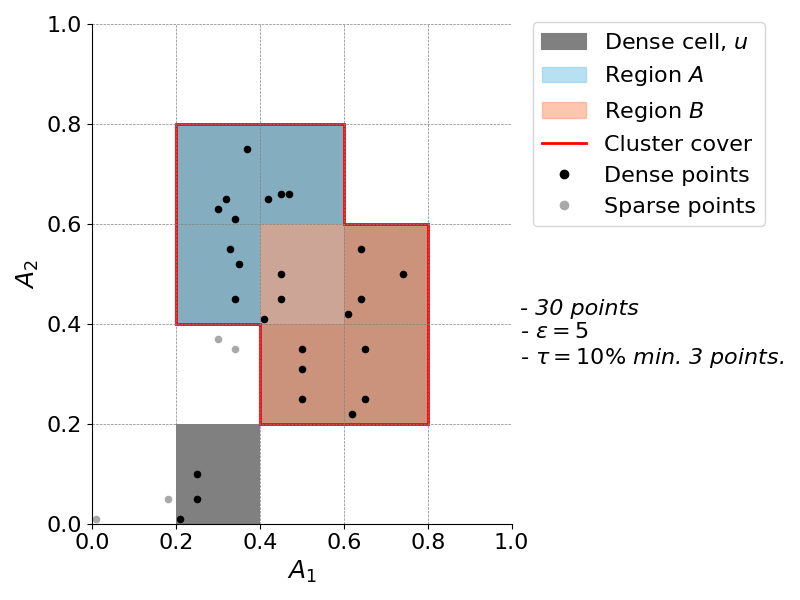
\includegraphics[width=0.4\textwidth]{figures/dense_cells_and_regions.png}
    \caption{2-dimensional space containing 8 DUs and despicting two overlapping dense regions $A$ and $B$.}
    \label{fig:dense_cells_and_regions}
    \vspace*{-0.5cm}
\end{figure}

\subsubsection{MAFIA}
MAFIA can be seen as an extension to CLIQUE and follows mostly the same procedure except from the following:
\begin{enumerate}
    \item Grid sizes are adaptive and automatically determined based on the data distribution.
    \item CDUs are formed using all combinations of the dimensions, that the DUs contains.
    \item Does not use the pruning technique as it could result in lost information, as already noted in \cite{clique}.
    \item Tries to parallelize the clustering process.
\end{enumerate}
Point 1 and 2 will be explained in more detail next.

\paragraph{Adaptive grids.}
The \textit{Adaptive} algorithm starts by divide each $A_i$ into high $n$-number of equal-sized windows (default $n = 1000$). Then, from left to right, two windows are merged together if their bin count are within a percentage of difference $\beta$ (input parameter). That means, a high $\beta$ value result in many merged windows, and vice-versa. If two windows are merged together, the highest bin count are assigned to the window, meaning the bin count that should be used to be compared with the next window. In other words, the algorithm does not use the total bin count of the two for the next comparison. Figure \ref{fig:adaptive_grids} shows an example before and after running the Adaptive algorithm. Having merged the windows, the algorithm finally determines a \textit{dense-level} for each of the windows, that determines how many points a window must contain for a unit to be dense, thus determines whether it should be a candidate for higher dimensional spaces. The dense-level is given by:
\begin{equation}
    \text{dense-level} = \frac{\alpha \cdot a\cdot |\mathcal{D}|}{D_i}
\end{equation}
where $a$ is the size of the window, $\alpha$ is the \textit{cluster dominance factor} (input parameter) and $D_i$ is the total range $A_i$ covers. Thus, a higher $\alpha$ results in a higher dense-level, and vice-versa.
\begin{figure}[H]
    \vspace*{-0.5cm}
    \centering
    \subfloat[][Uncombined windows]{%
        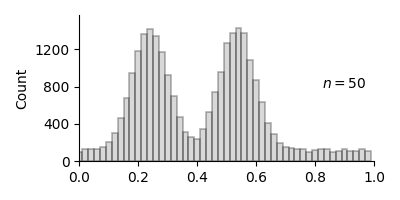
\includegraphics[width=0.4\textwidth]{figures/uncombined_histogram.png}\label{fig:uncombined_bins}}~~~~
    \subfloat[][Combineed windows]{%
        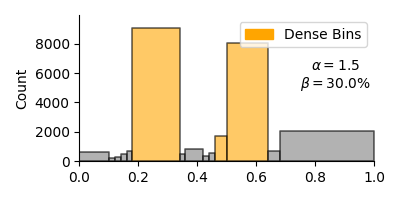
\includegraphics[width=0.4\textwidth]{figures/combined_histogram.png}\label{fig:combined_bins}}~~~~
    \caption{Illustration of the adaptive grids computation.}
    \label{fig:adaptive_grids}
    \vspace*{-0.5cm}
\end{figure}

\paragraph{CDU Generation.}
MAFIA uses the following definition when forming CDUs in $k$-dimensional space:
\begin{definition}
    CDUs in $k$-dimensional space are formed by merging DUs from the $(k-1)$-dimensional space that share \textit{any} $(k-2)$ attributes.
\end{definition}
Indeed, this results in a high time complexity of $O(Ndu^2)$, where $Ndu$ is the number of DUs. To control this complexity, CLIQUE restricts merging two DUs that share only the first $(k-2)$ dimensions. MAFIA, however, allows a broader merging strategy, combining DUs that share any $(k-2)$ dimensions. MAFIA can afford this approach because its adaptive grids reduce the number of DUs, effectively controlling the number of comparisons. This flexibility allows MAFIA to achieve a balance between efficiency and more comprehensive cluster detection.

An example illustrating the advantage of merging DUs that share any $(k-2)$ dimensions is shown in the following Table \ref{tab:cdu}. Here, 3 DUs are provided to the a 4-dimensional space. Both CLIQUE and MAFIA would form a 4-dimensional CDU based on DU1 and DU2, as they share the \textit{first} two dimensions. However, only MAFIA would form a CDU based on DU1 and DU3, since it allows merging based on \textit{any} dimensions.
\begin{table}[H]
    \vspace*{-0.5cm}
    \centering
    \begin{tabular}{|c|c|c|}
        \hline
        DU1 & DU2 & DU3 \\
        \hline
        $\{1, 2, 3\}$ & $\{1, 2, 4\}$ & $\{2, 3, 4\}$ \\
        \hline
    \end{tabular}
    \vspace*{0.2cm}
    \caption{Illustration of forming a CDU in 4-dimensional space. The number given in each DU represents the dimensions it contains.}
    \label{tab:cdu}
    \vspace*{-0.5cm}
\end{table}

\subsection{Density-Connected approach}
A drawback of grid-based methods is that the quality of clustering depends on the positiong of the grids. In Figure \ref{fig:dense_cells_and_regions}, we see that the due to the rigid grid structure we might miss cluster points, that is point not in a dense cell. This problem especially occurs for clusters that are not of rectangular shapes thus, allowing to detect clusters of arbitrary shapes and orientations. One way to address this issue is to a density-connected algorithm, which uses the neighbourhood of points to determine clusters. One such algorithm is SUBCLU.

\subsubsection{SUBCLU}
SUBCLU extends the principles of the well-known DBSCAN algorithm \cite{dbscan} to higher dimensions by leveraging Lemma \ref{lem:mono}, which guides the search for clusters across subspaces.

The algorithm begins by applying DBSCAN to each attribute $A_i$ separately in 1-dimensional subspaces. It identifies dense regions using two input parameters: $\varepsilon$ which defines the neighborhood radius for points to be considered neighbors, and $m$, the minimum number of points required for a point to qualify as a \textit{core point}. If a point is not a core point but lies within $\varepsilon$ of a core point, it is classified as a \textit{border point}. Points that are neither core nor border points are treated as \textit{noise}.

A \textit{density-connected set} consists of core points that are linked through other core points, and border points that extend the cluster but do not meet the density criteria themselves. These border points are connected to the cluster via core points within their $\varepsilon$-neighborhood. A cluster is thus defined as the union of all density-connected sets, including both core and border points.

SUBCLU follows a bottom-up approach: after detecting clusters in 1-dimensional subspaces, it combines $k$-dimensional subspaces that share $(k-1)$ dimensions to generate candidate $(k+1)$-dimensional subspaces. DBSCAN is reapplied to these candidate subspaces using the same $\varepsilon$ and $m$ values to verify whether the clusters found in lower-dimensional subspaces persist as new dimensions are added. Lemma \ref{lem:mono} helps to prune the search space efficiently, allowing SUBCLU to prune subspaces where no clusters are detected, thus reducing unnecessary computations.

An example is shown in Figure \ref{fig:subclu}, where SUBCLU identifies a cluster in a 2-dimensional subspace consiting of 6 points. Note that if $minpts = 2$ instead of 3 it identifies two core points.
\begin{figure}[H]
    \vspace*{-0.5cm}
    \centering
    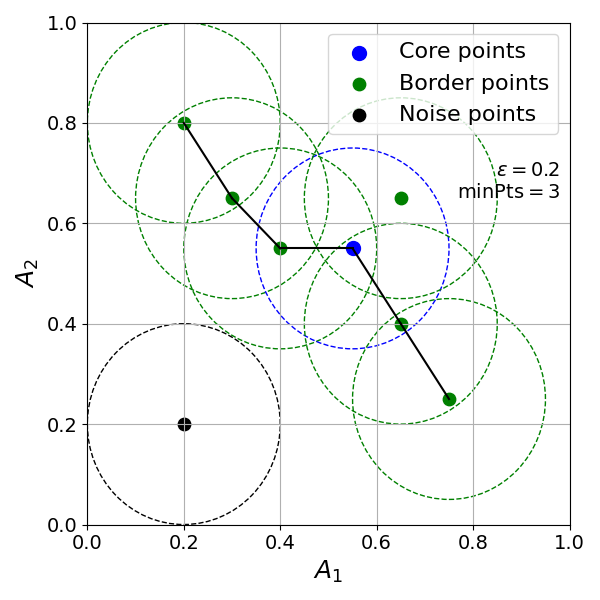
\includegraphics[width=0.35\textwidth]{figures/subclu.png}
    \caption{Illustration of SUBCLU identifying a cluster in a 2-dimensional subspace.}
    \label{fig:subclu}
    \vspace*{-0.5cm}
\end{figure}